\subsection{Questions}

In order for the interview to go smoothly it is important to define the questions beforehand. The questions will be based on the research framework and the evaluation criteria. The interviews will be conducted by Jessie Liauw A Fong and the interviewee will be a software architect.

Questions about how they view software architecture:
\begin{itemize}
  \item What is software architecture?
  \item What is your company the main job of a software architect?
  \item Which with kind of architectures have you worked?
  \item What is the biggest pitfall when implementing a new architecture?
  \item How do you decide which architecture is best of a certain project?
  \item What is the architecture that you implement in most of your projects? (Frontend and backend)
\end{itemize}

Questions about how they view modularity:
\begin{itemize}
  \item What is the first thing that you think of when I say modular architecture?
  \item What are the most upcoming architectures that are focused on modularity in your opinion?
  \item Which programming languages do you think compliments a modular architecture best?
  \item
\end{itemize}

Questions about the chosen architecture and method:
\begin{itemize}
  \item What do you think of the image about how I went my way in choosing the right architecture?
  \item What is your opinion about domain driven design
  \item Have you ever heard of modular monolith
\end{itemize}

\begin{figure}[H]
	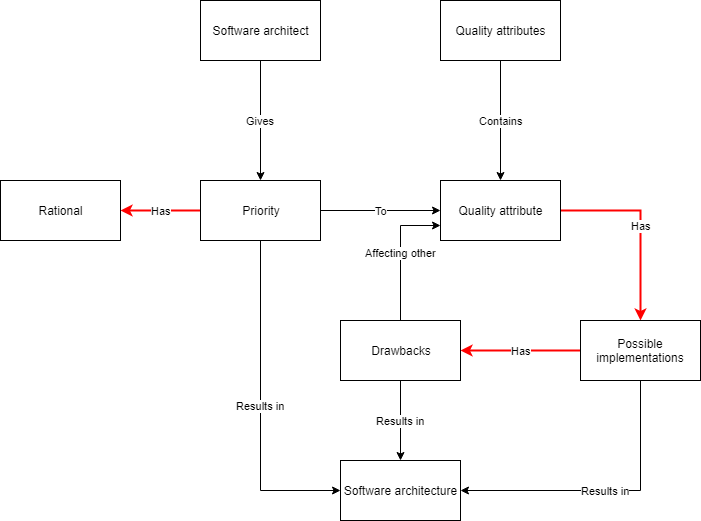
\includegraphics[width=\linewidth]{creating_architecture.png}
	\caption{How a software architecture is chosen}
\end{figure}
